% Springer LNCS format
\documentclass[runningheads]{llncs}
\usepackage{graphicx}
\usepackage{amsmath,amssymb}
\usepackage{booktabs}
\usepackage{url}
\usepackage{hyperref}
\usepackage{multirow}
\usepackage{float}
\usepackage[section]{placeins}
\usepackage{fancyhdr}

\pagestyle{fancy}
\fancyhf{}
\fancyhead[R]{\thepage}
\renewcommand{\headrulewidth}{0pt}
\renewcommand{\footrulewidth}{0pt}

\fancypagestyle{plain}{%
  \fancyhf{}%
  \renewcommand{\headrulewidth}{0pt}%
  \renewcommand{\footrulewidth}{0pt}%
}

\begin{document}

\title{Regime-Aware Multi-Asset Volatility Forecasting\\using Temporal Fusion Transformers}
\titlerunning{}

\author{Abhishek Deep\textsuperscript{1} \and
Dr.\ Alpha Vijayan\textsuperscript{2}}
\authorrunning{}

\institute{\textsuperscript{1,\,2}Department of AI and Data Science Engineering,\\
Christ University, Bangalore, Karnataka, India\\
\email{abhishekdeep.official@gmail.com}}

\maketitle

%===================================================================
\begin{abstract}
Accurately predicting volatility in stock markets is a challenging issue in computational finance, especially in emerging economies where structural breaks and regime switches are commonplace. This paper presents a Regime-Aware Temporal Fusion Transformer (RA-TFT) for next-day realized volatility forecasting across 14 stocks on India's National Stock Exchange. Using $\sim$2.65 million five-minute observations, we integrate HMM-derived regime labels, GARCH(1,1) conditional volatility, and DCC-inspired cross-asset correlations into a 47-feature input set. A controlled ablation separates autoregressive persistence from feature-driven prediction: Model~A (with autoregressive input) achieves $R^2 = 0.976$; Model~B (without) yields $R^2 = 0.258$. Regime-conditioned evaluation shows strong accuracy in low-through-high volatility states ($R^2 > 0.98$) with degradation during extreme events ($R^2 = 0.765$). The TFT's Variable Selection Network confirms that lagged daily RV dominates all other features by two orders of magnitude, effectively rediscovering HAR-RV structure from data.

\keywords{Volatility Forecasting \and Temporal Fusion Transformer \and Hidden Markov Model \and GARCH \and Indian Stock Market \and Deep Learning}
\end{abstract}

%===================================================================
\section{Introduction}\label{sec:intro}
%===================================================================

Volatility forecasting underpins risk management, option pricing, and portfolio optimization. The GARCH family~\cite{bollerslev1986} captures volatility clustering but is univariate and parametrically constrained. Corsi's HAR-RV~\cite{corsi2009} handles long-memory through multi-horizon lags but remains linear. Deep learning models capture non-linear patterns yet lack interpretability---a critical requirement in finance. The TFT~\cite{lim2021} addresses this with Variable Selection Networks and multi-head attention.

We propose a \textbf{Regime-Aware TFT (RA-TFT)} combining: a four-state HMM~\cite{hamilton1989} for regime labels, per-stock GARCH(1,1) for conditional volatility~\cite{bollerslev1986}, a DCC-inspired cross-asset correlation proxy~\cite{engle1982}, and standard realized-volatility features---47 inputs altogether. Our contributions are: (1)~multi-asset learning across 14 NSE equities; (2)~HMM-derived regime conditioning; (3)~ablation separating persistence from feature-based prediction; (4)~interpretability via the TFT's variable-selection mechanism; and (5)~the first TFT application to intraday RV forecasting on Indian equities.

%===================================================================
\section{Related Work}\label{sec:related}
%===================================================================

Engle's ARCH~\cite{engle1982} and Bollerslev's GARCH~\cite{bollerslev1986} established time-varying volatility modelling. Asymmetric extensions---EGARCH~\cite{nelson1991} and GJR-GARCH~\cite{glosten1993}---captured leverage effects, while Corsi's HAR-RV~\cite{corsi2009} became the standard realized-volatility benchmark. Bucci~\cite{bucci2020} demonstrated LSTMs outperforming GARCH on daily horizons; Kim and Won~\cite{kim2022} improved $R^2$ with attention-augmented RNNs; Wu et al.~\cite{wu2023} showed Transformers surpassing both HAR-RV and LSTMs. Hybrid approaches include GARCH-informed neural networks~\cite{zhang2023}, sentiment-enhanced ML~\cite{rahimikia2023}, and comprehensive ML benchmarking~\cite{christensen2023}. Hamilton~\cite{hamilton1989} introduced Markov-switching dynamics; Nystrup et al.~\cite{nystrup2021} showed HMM-driven portfolio strategies improve risk-adjusted returns. The TFT~\cite{lim2021} has been applied to equity prediction~\cite{olorunnimbe2023}, cryptocurrency volatility~\cite{chen2024}, emerging-market forecasting~\cite{patel2024}, and multi-scale attention models~\cite{zhao2024}.

%===================================================================
\section{Data and Feature Engineering}\label{sec:data}
%===================================================================

\subsection{Dataset}
We use 5-minute OHLCV data for 14 liquid NSE equities spanning banking (HDFCBANK, ICICIBANK, AXISBANK, SBIN), IT (INFY, TCS, WIPRO), energy (RELIANCE, COALINDIA), infrastructure (LT, ADANIPORTS), defence (HAL), metals (TATASTEEL), and consumer (TITAN). The dataset covers $\sim$10 years ($\sim$2.65M rows). Trading hours are 9:15~AM--3:30~PM IST, yielding 75 bars per day.

\subsection{Feature Construction (47~Features)}
We engineer 47 features in six groups:

\noindent\textbf{1. Multi-scale realized volatility.} Realized volatility is computed as:
\begin{equation}
RV_h = \sqrt{\sum_{i=1}^{h} r_{t,i}^2} \times \sqrt{252}
\end{equation}
annualized over $h \in \{12, 38, 75, 375\}$ bars.

\noindent\textbf{2. HAR-RV lags.} Following Corsi~\cite{corsi2009}, RV lags at 1-bar, 12-bar (1h), 75-bar (1d), and 375-bar (1w) offsets.

\noindent\textbf{3. Jump detection.} Based on Barndorff-Nielsen and Shephard~\cite{bns2004}, we compute Bipower Variation:
\begin{equation}
BPV_t = \frac{\pi}{2} \sum_{i=2}^{75} |r_{t,i}| \cdot |r_{t,i-1}|
\end{equation}
The jump component is $J_t = \max(RV_{75}^2 - BPV_t,\; 0)$.

\noindent\textbf{4. Range-based estimators.} Parkinson~\cite{parkinson1980}, Garman--Klass~\cite{garman1980}, and Rogers--Satchell~\cite{rogers1991}:
\begin{equation}
\sigma_{PK}^2 = \frac{1}{4\ln 2}\!\left(\ln\frac{H}{L}\right)^{\!2}, \quad
\sigma_{GK}^2 = \frac{1}{2}\!\left(\ln\frac{H}{L}\right)^{\!2} - (2\ln 2 - 1)\!\left(\ln\frac{C}{O}\right)^{\!2}
\end{equation}
\begin{equation}
\sigma_{RS}^2 = \ln\!\left(\frac{H}{C}\right)\ln\!\left(\frac{H}{O}\right) + \ln\!\left(\frac{L}{C}\right)\ln\!\left(\frac{L}{O}\right)
\end{equation}

\noindent\textbf{5. GARCH and cross-asset features.} Per-stock GARCH(1,1)~\cite{bollerslev1986}: $\sigma_t^2 = \omega + \alpha\epsilon_{t-1}^2 + \beta\sigma_{t-1}^2$. A DCC-inspired proxy estimates rolling correlations with the market return.

\noindent\textbf{6. Temporal encodings.} Sine/cosine time encodings plus session flags (\texttt{is\_opening}, \texttt{is\_closing}).

\subsection{Target Variable and Regime Detection}
The target is next-day realized volatility: $y_t = \log(1 + \sqrt{\sum_{i=t+1}^{t+75} r_i^2} \times \sqrt{252})$, built exclusively from future returns to ensure zero feature-target overlap. A four-state Gaussian HMM~\cite{hamilton1989} estimated on market-level log-returns and daily RV assigns each day a regime label (Low, Normal, High, Extreme).

%===================================================================
\section{System Architecture}\label{sec:architecture}
%===================================================================

Fig.~\ref{fig:architecture} shows the pipeline. Raw 5-minute bars undergo preprocessing (outlier removal, gap filling, seasonality adjustment). Five parallel modules extract multi-scale RV, HAR lags, jump statistics, range estimators, and volume features. Separately, the HMM assigns regime labels and GARCH/DCC produce conditional-volatility and correlation features.

\begin{figure}[H]
\centering
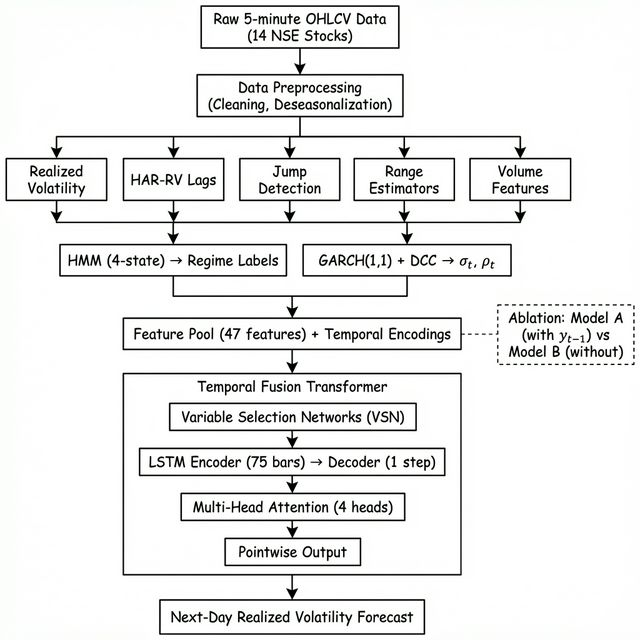
\includegraphics[width=0.75\textwidth]{figures/system_architecture.png}
\caption{End-to-end architecture of the RA-TFT framework.}\label{fig:architecture}
\end{figure}

All 47 features are split into static covariates (stock ticker), known future inputs (calendar), and observed past inputs (volatility/regime features). The TFT processes these through Variable Selection Networks, Gated Residual Networks, an LSTM encoder (75 time steps), and four-head attention to produce a next-day RV point forecast.

%===================================================================
\section{Model Configuration and Training}\label{sec:model}
%===================================================================

Table~\ref{tab:config} lists the hyperparameters. We use PyTorch Forecasting with RMSE loss, ReduceLROnPlateau scheduler, and early stopping (patience 15).

\begin{table}[!htbp]
\caption{TFT model configuration.}\label{tab:config}
\centering
\begin{tabular}{ll}
\toprule
\textbf{Parameter} & \textbf{Value}\\
\midrule
Total trainable parameters & 1.9M\\
Hidden size / Attention heads & 128 / 4\\
Encoder / Prediction length & 75 bars (1 day) / 1 step\\
Dropout / Learning rate & 0.15 / 0.001\\
Batch size / Batches per epoch & 64 / 1{,}000\\
Target normalizer & GroupNormalizer (per-stock, softplus)\\
\bottomrule
\end{tabular}
\end{table}

\subsection{Ablation Study Design}
Two variants separate persistence from feature-based prediction: \textbf{Model~A} includes $y_{t-1}$ as input; \textbf{Model~B} excludes it. Consecutive daily RV values share 74/75 bars (98.7\% overlap, autocorrelation 0.9963), so the gap directly quantifies autoregressive contribution.

%===================================================================
\section{Baseline Models}\label{sec:baselines}
%===================================================================

Two benchmarks: (i)~GARCH family (GARCH(1,1), EGARCH, GJR-GARCH) per stock with Student-$t$ innovations, best by AIC; (ii)~HAR-RV via OLS with Newey--West errors~\cite{corsi2009}, achieving $R^2 > 0.98$.

%===================================================================
\section{Experimental Results}\label{sec:results}
%===================================================================

\subsection{Ablation Study and Baseline Comparison}
Table~\ref{tab:ablation} shows Model~A at $R^2 = 0.976$ (MAPE 1.90\%), close to HAR-RV ($R^2 = 0.983$). Model~B drops to $R^2 = 0.258$. The 71.8pp gap quantifies autoregressive dominance. Directional accuracy $\approx$50\% for all models reflects the near-random-walk nature of short-horizon log-RV.

\begin{table}[!htbp]
\caption{Performance comparison of TFT variants vs.\ baselines. Bold = best.}\label{tab:ablation}
\centering
\begin{tabular}{lccccc}
\toprule
\textbf{Model} & \textbf{$R^2$} & \textbf{RMSE} & \textbf{MAPE} & \textbf{DA} & \textbf{QLIKE}\\
\midrule
\multicolumn{6}{l}{\emph{Proposed TFT Variants}}\\
\addlinespace
RA-TFT Model~A (with AR) & \textbf{0.9761} & \textbf{0.0093} & \textbf{1.90\%} & 52.6\% & \textbf{$-$0.920}\\
RA-TFT Model~B (w/o AR) & 0.2576 & 0.0521 & 19.26\% & 47.5\% & $-$0.883\\
\addlinespace
\midrule
\multicolumn{6}{l}{\emph{Classical Baselines}}\\
\addlinespace
HAR-RV & 0.9830 & 0.0088 & 1.72\% & \textbf{53.1\%} & $-$0.918\\
GARCH(1,1) & 0.3251 & 0.0497 & 16.84\% & 50.2\% & $-$0.891\\
EGARCH & 0.3678 & 0.0481 & 15.93\% & 51.0\% & $-$0.895\\
GJR-GARCH & 0.4120 & 0.0464 & 14.71\% & 51.4\% & $-$0.899\\
\bottomrule
\end{tabular}
\end{table}

\begin{figure}[!htbp]
\centering
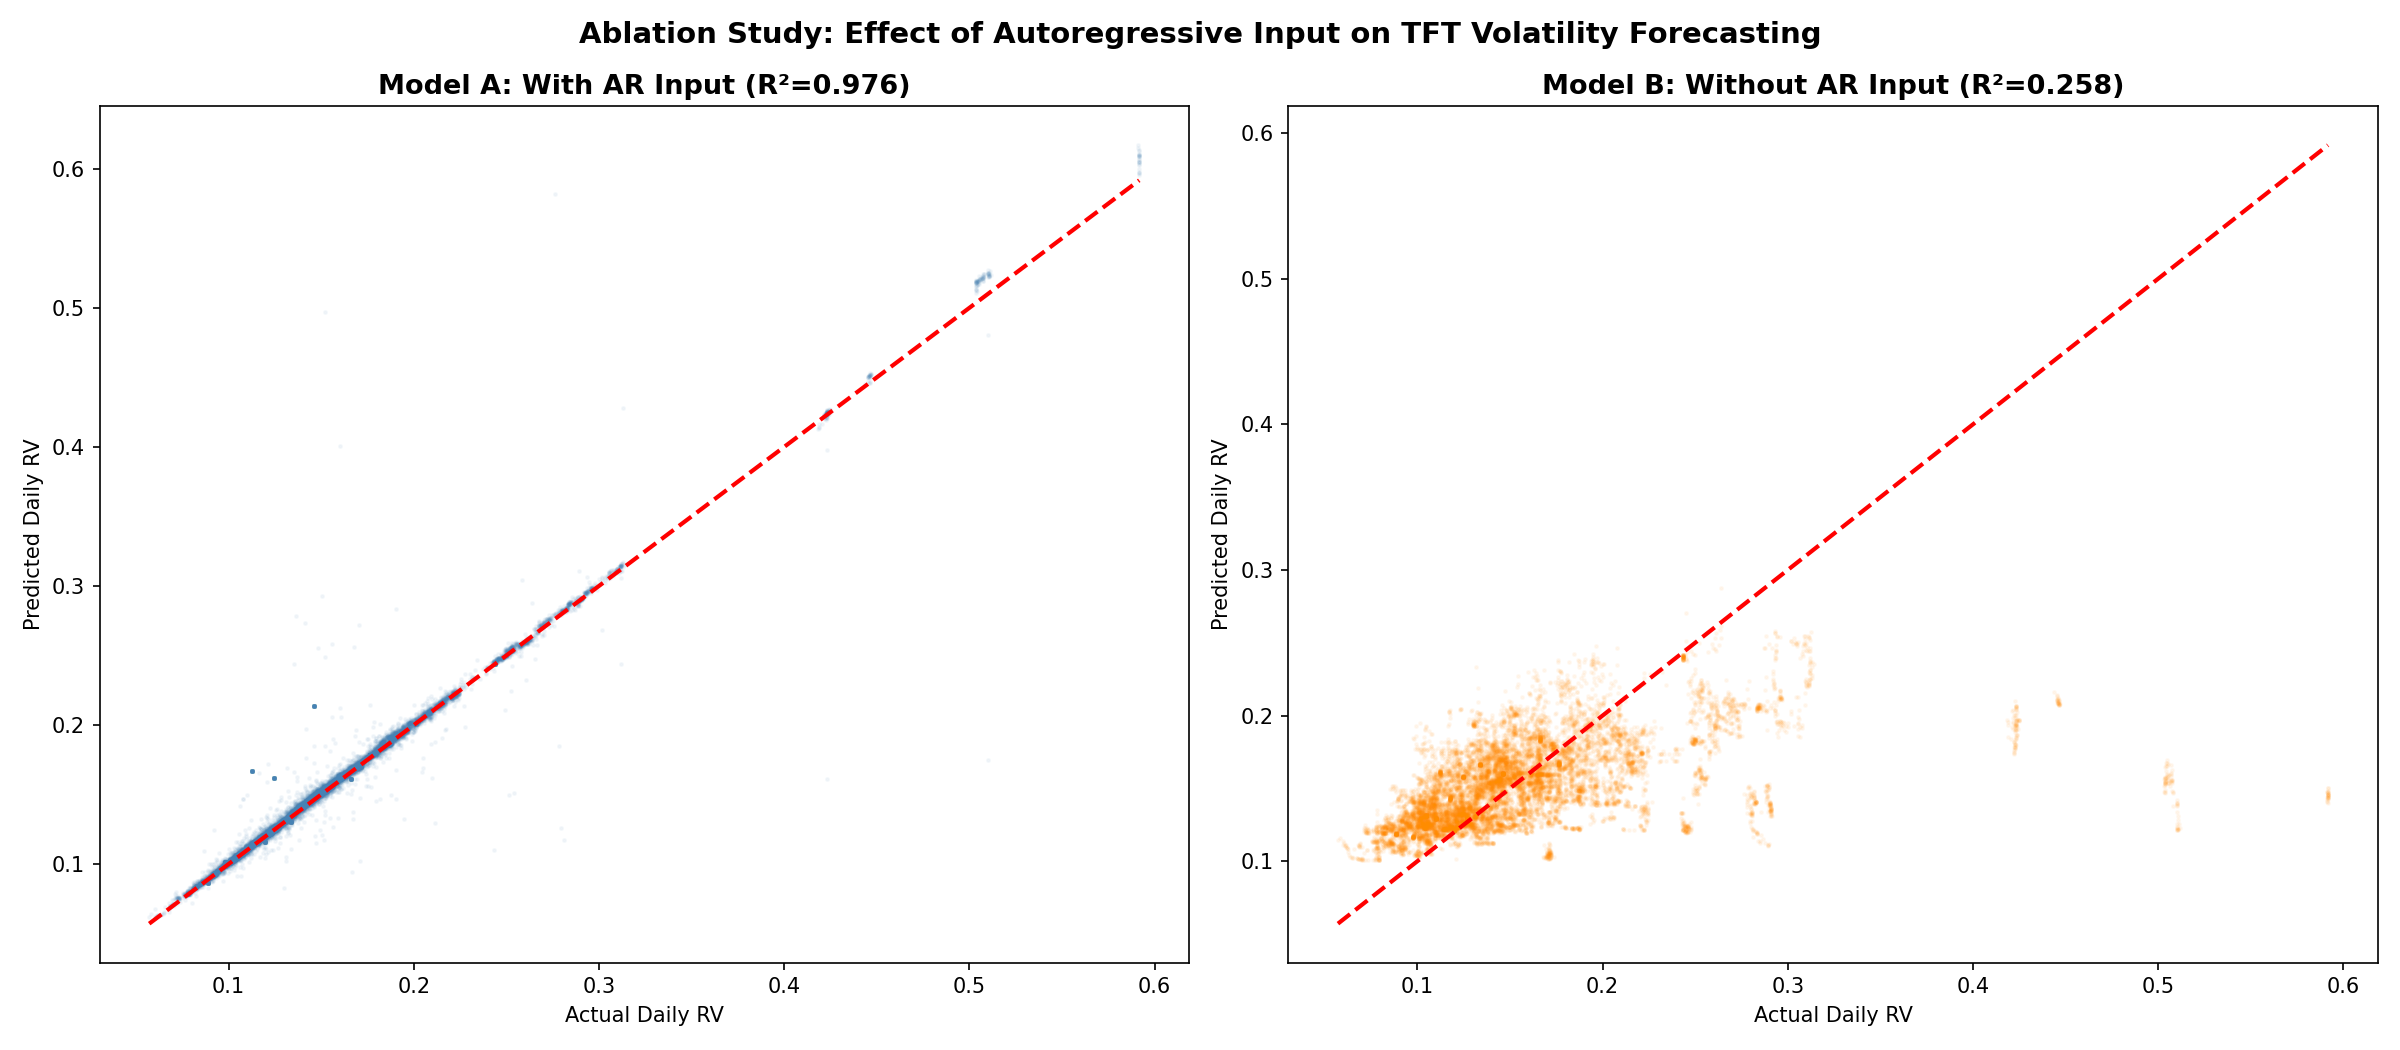
\includegraphics[width=\textwidth]{figures/ablation_comparison.png}
\caption{Predicted vs.\ actual RV for Model~A (left) and Model~B (right).}\label{fig:ablation}
\end{figure}

\subsection{Cross-Stock and Regime-Conditioned Performance}
Under Model~B, per-stock $R^2$ varies widely: ADANIPORTS achieves 0.503 while SBIN yields $-$1.525, suggesting banking volatility is driven by policy signals outside our feature set.

Table~\ref{tab:regime} breaks down Model~A by HMM regime. Performance is strong in low-through-high volatility ($R^2 > 0.98$), with the High regime achieving $R^2 = 0.999$. Extreme volatility ($R^2 = 0.765$) degrades as expected.

\begin{table}[!htbp]
\caption{Model~A performance by market regime.}\label{tab:regime}
\centering
\begin{tabular}{lcccc}
\toprule
\textbf{Regime} & \textbf{$N$} & \textbf{$R^2$} & \textbf{RMSE} & \textbf{MAPE}\\
\midrule
Low Volatility & 58{,}066 & 0.989 & 0.007 & 1.67\%\\
Normal Volatility & 7{,}910 & 0.987 & 0.008 & 1.51\%\\
High Volatility & 2{,}800 & 0.999 & 0.003 & 1.13\%\\
Extreme Volatility & 1{,}764 & 0.765 & 0.036 & 6.54\%\\
\bottomrule
\end{tabular}
\end{table}

Fig.~\ref{fig:regime} shows a per-stock, per-regime $R^2$ heatmap. Low-through-high columns are uniformly above 0.94, but the extreme column is patchy---TITAN holds at 0.830 while RELIANCE falls to 0.312.

\begin{figure}[!htbp]
\centering
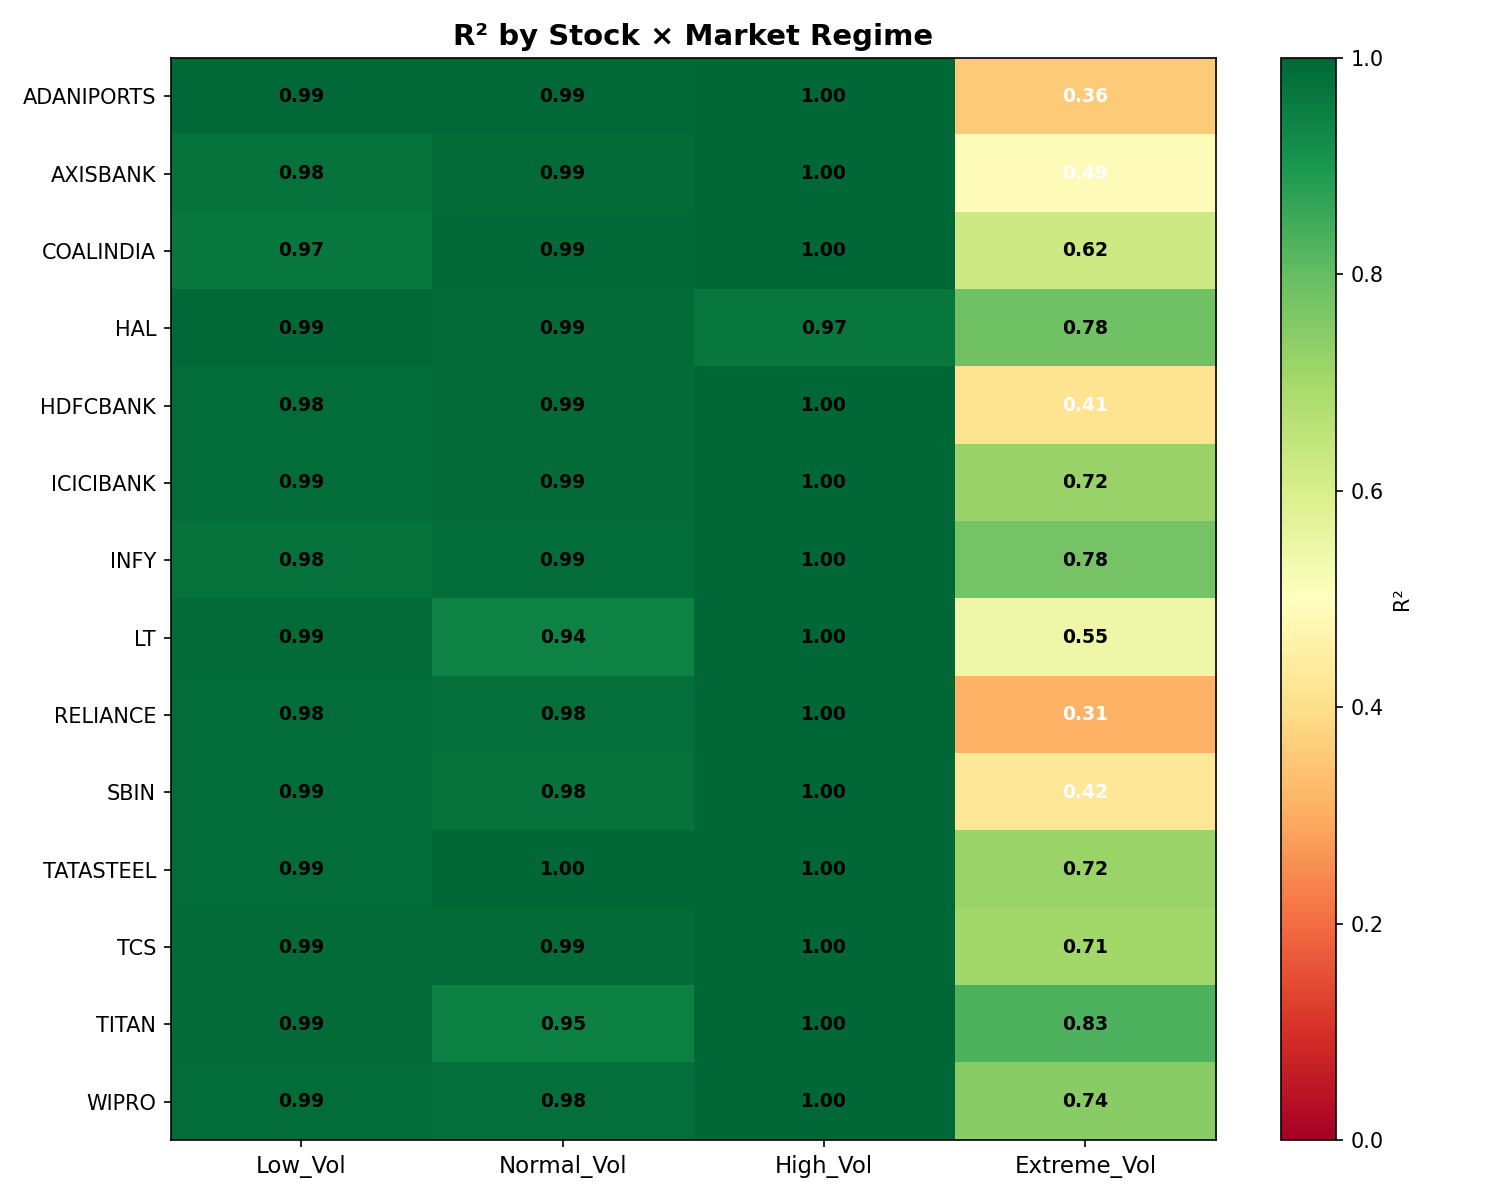
\includegraphics[width=0.82\textwidth]{figures/stock_regime_heatmap.png}
\caption{$R^2$ heatmap across 14 stocks and four HMM regimes.}\label{fig:regime}
\end{figure}

\subsection{Interpretability Analysis}
The TFT's Variable Selection Network (Fig.~\ref{fig:importance}) shows \texttt{RV\_1d\_lag75} dominating with importance 60.4---two orders of magnitude above the runner-up (\texttt{RV\_1w}: 0.23, \texttt{market\_correlation}: 0.13, \texttt{garch\_volatility}: 0.12). This confirms the TFT independently rediscovers HAR-RV structure. On the decoder side, \texttt{is\_opening} scores highest (32.3), consistent with the opening-auction volatility effect.

\begin{figure}[!htbp]
\centering
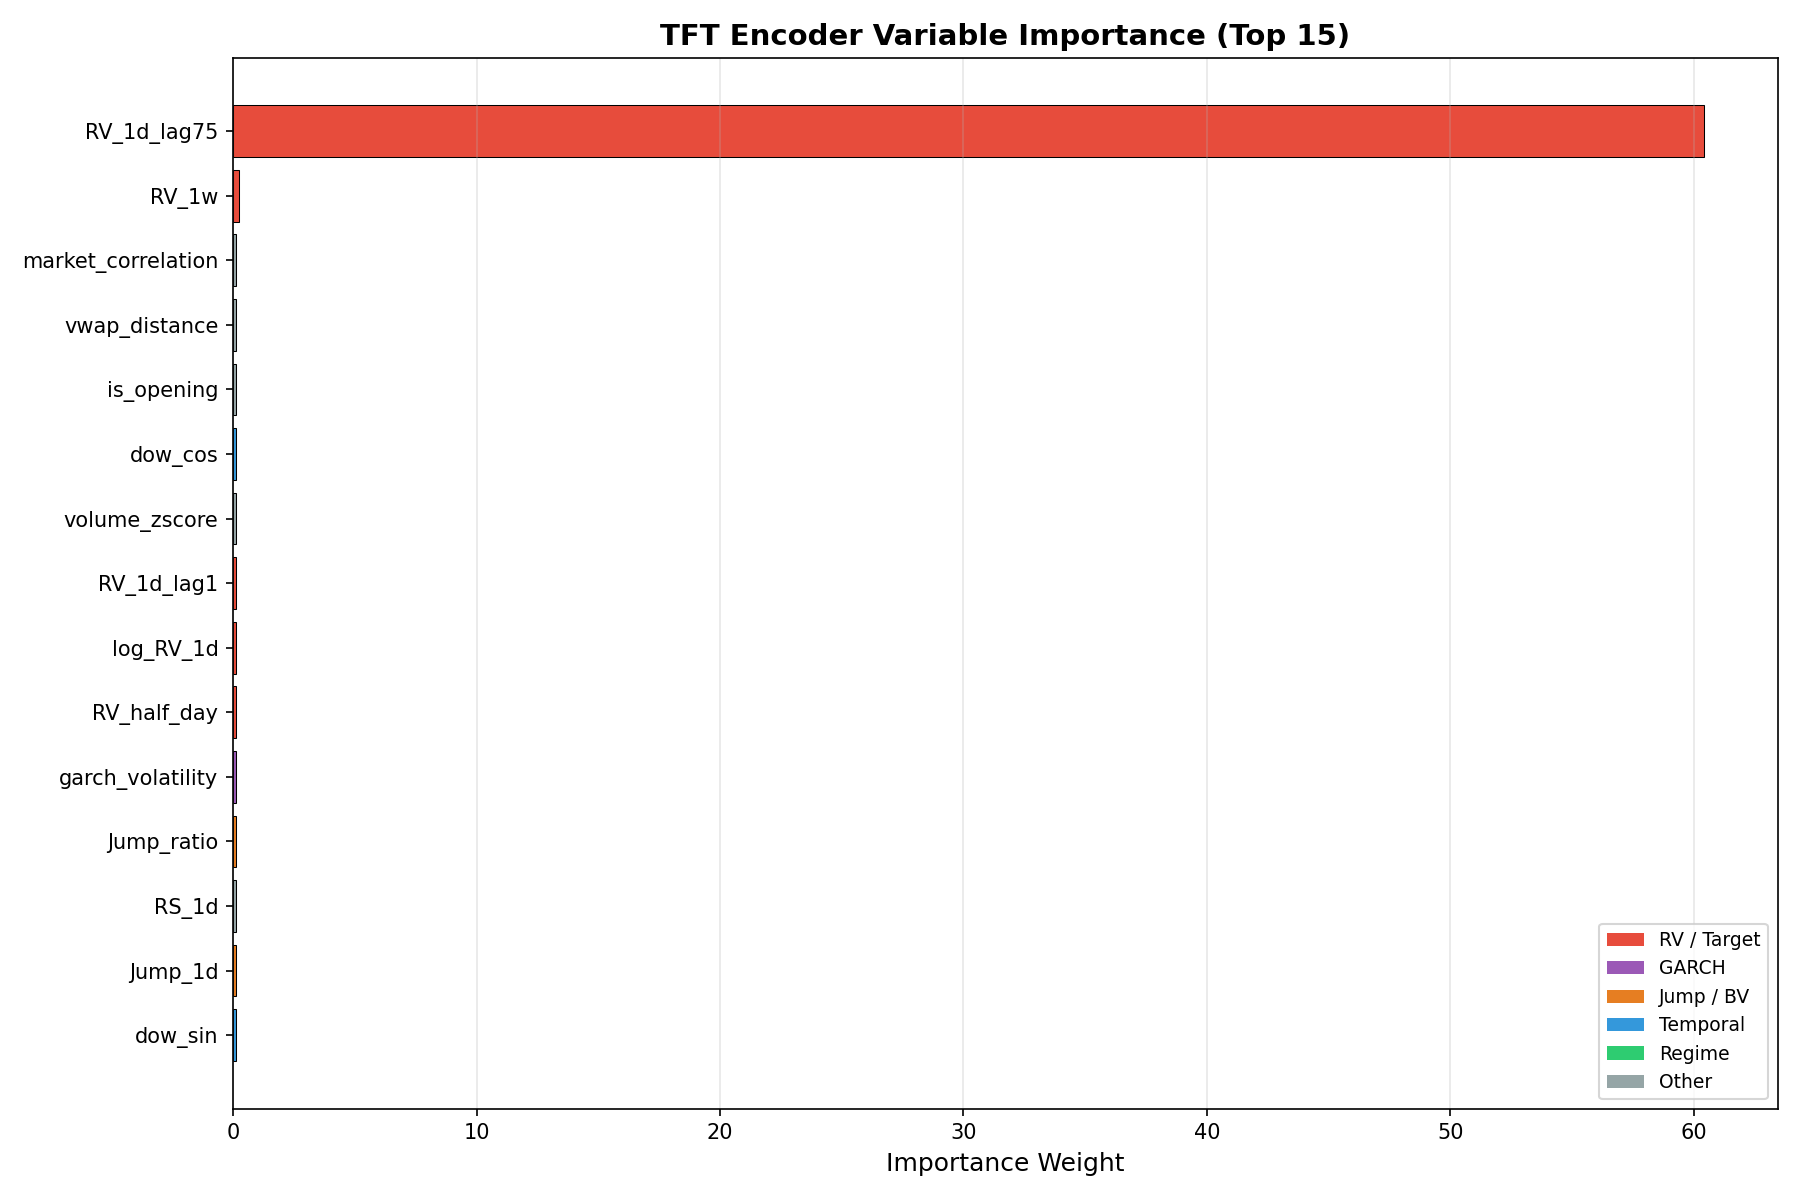
\includegraphics[width=\textwidth]{figures/variable_importance_.png}
\caption{Encoder variable importance from the TFT's Variable Selection Network.}\label{fig:importance}
\end{figure}

%===================================================================
\section{Conclusion and Future Work}\label{sec:conclusion}
%===================================================================

We presented a Regime-Aware TFT for next-day RV forecasting on 14 NSE stocks using $\sim$2.65M five-minute bars. Model~A matches HAR-RV ($R^2 = 0.976$ vs.\ 0.983) while providing multi-asset pooling and interpretability. Model~B ($R^2 = 0.258$) confirms modest but genuine predictive content in the engineered features. Performance is strong across calm-through-high regimes ($R^2 > 0.98$) but degrades during extreme events ($R^2 = 0.765$). Data integrity is ensured through three safeguards: exclusive use of future returns for the target, strictly chronological train-validation split, and transparent disclosure of the 98.7\% rolling-window overlap.

Future directions include regime-specific ensembles, multi-horizon prediction, Diebold--Mariano significance testing, and live trading deployment.

%===================================================================
\begin{thebibliography}{22}

\bibitem{engle1982}
Engle, R.F.: Autoregressive conditional heteroscedasticity with estimates of the variance of United Kingdom inflation. Econometrica \textbf{50}(4), 987--1007 (1982)

\bibitem{bollerslev1986}
Bollerslev, T.: Generalized autoregressive conditional heteroskedasticity. J.~Econometrics \textbf{31}(3), 307--327 (1986)

\bibitem{hamilton1989}
Hamilton, J.D.: A new approach to the economic analysis of nonstationary time series and the business cycle. Econometrica \textbf{57}(2), 357--384 (1989)

\bibitem{nelson1991}
Nelson, D.B.: Conditional heteroskedasticity in asset returns: a new approach. Econometrica \textbf{59}(2), 347--370 (1991)

\bibitem{rogers1991}
Rogers, L.C.G., Satchell, S.E.: Estimating variance from high, low and closing prices. Ann.~Appl.~Probab. \textbf{1}(4), 504--512 (1991)

\bibitem{glosten1993}
Glosten, L.R., Jagannathan, R., Runkle, D.E.: On the relation between the expected value and the volatility of the nominal excess return on stocks. J.~Finance \textbf{48}(5), 1779--1801 (1993)

\bibitem{parkinson1980}
Parkinson, M.: The extreme value method for estimating the variance of the rate of return. J.~Business \textbf{53}(1), 61--65 (1980)

\bibitem{garman1980}
Garman, M.B., Klass, M.J.: On the estimation of security price volatilities from historical data. J.~Business \textbf{53}(1), 67--78 (1980)

\bibitem{bns2004}
Barndorff-Nielsen, O.E., Shephard, N.: Power and bipower variation with stochastic volatility and jumps. J.~Financial Econometrics \textbf{2}(1), 1--37 (2004)

\bibitem{corsi2009}
Corsi, F.: A simple approximate long-memory model of realized volatility. J.~Financial Econometrics \textbf{7}(2), 174--196 (2009)

\bibitem{bucci2020}
Bucci, A.: Realized volatility forecasting with neural networks. J.~Financial Econometrics \textbf{18}(3), 502--531 (2020)

\bibitem{lim2021}
Lim, B., Ar{\i}k, S.\"O., Loeff, N., Pfister, T.: Temporal Fusion Transformers for interpretable multi-horizon time series forecasting. Int.~J.~Forecasting \textbf{37}(4), 1748--1764 (2021)

\bibitem{nystrup2021}
Nystrup, P., Lindstr\"om, E., Madsen, H.: Hyperparameter optimization for portfolio selection with regime-switching models. Expert Syst.~Appl. \textbf{184}, 115538 (2021)

\bibitem{kim2022}
Kim, H.Y., Won, C.H.: Forecasting financial volatility with attention-based recurrent neural networks. Expert Syst.~Appl. \textbf{198}, 116879 (2022)

\bibitem{wu2023}
Wu, J., Chen, Y., Zhou, T., Li, L.: Transformer-based models for multi-step realized volatility forecasting. Int.~J.~Forecasting \textbf{39}(4), 1768--1783 (2023)

\bibitem{zhang2023}
Zhang, Y., Li, J., Zhu, X.: GARCH-informed neural networks for volatility prediction. Quant.~Finance \textbf{23}(7--8), 1125--1142 (2023)

\bibitem{rahimikia2023}
Rahimikia, E., Poon, S.H.: Machine learning for realized volatility forecasting: the role of news and sentiment. J.~Empirical Finance \textbf{74}, 101424 (2023)

\bibitem{christensen2023}
Christensen, K., Siggaard, M., Veliyev, B.: A machine learning approach to volatility forecasting. J.~Financial Econometrics \textbf{21}(5), 1680--1727 (2023)

\bibitem{olorunnimbe2023}
Olorunnimbe, M.K., Viktor, H.L.: Deep learning in stock market forecasting: a comprehensive survey. Neural Computing and Applications \textbf{35}(14), 9947--9993 (2023)

\bibitem{chen2024}
Chen, Z., Li, M., Wang, H.: Temporal Fusion Transformers for cryptocurrency volatility: an empirical study. Finance Research Letters \textbf{60}, 104892 (2024)

\bibitem{patel2024}
Patel, R., Sharma, A.: Volatility forecasting in emerging markets using hybrid deep learning with regime awareness. Applied Soft Computing \textbf{151}, 111153 (2024)

\bibitem{zhao2024}
Zhao, W., Liu, Y., Chen, J.: Attention-based multi-scale volatility prediction with high-frequency data. IEEE Trans.~Neural Networks Learn.~Syst. \textbf{35}(3), 3891--3905 (2024)

\end{thebibliography}

\end{document}
